\section{Neural network implementation and models} **COMBINE THIS TO NEXT SECTION**
In this project the deep learning method is used to classify the pain maps and gender by determined outputs. The data is a set of 2D-images combined with gender and the outputs, pain intensity and duration. For classification purpose supervised convolutional neural network is used followed by fully-connected layers at the end. This architecture is chosen to the interest of morphology and location of the pain. The models are trained and tested on a single computer with GPU and ran on Python programming language with Keras library and Tensorboard tool for visualizing results. Specifications of hardware and software are described in detail in section 4.2.
WE STOPPED HERE!!!!!!!!!!!!*****
\noindent
The architecture of model is presented in PICTURE(If nesceserry). From the higher point of view, the model can be architecturally splitted into two main parts. Feature extraction part, where convolutional and pooling layers alternates in order to extract the most important features out of the image. Second part is called classification, where computed feature maps will be assigned to particular class of the output layer. In order to obtain a better accuracy of deep learning classifier, methods like activation function, regulation and optimization will be used within the layers.

\noindent
Activation function is used to fit nonlinear patterns in the data and to control when the node in the model should be considered as an active or not.  In this project “Rectified linear unit” (ReLu) activation function will be used as given since this is the most common for nueral network (equation)  \citep{Goodfellow2016}.

\noindent
Regulation is a method for restricting model from overfitting. The most common which is used in this project is called dropout. It randomly omitts the fixed percentage amount of neurons in order to significantly improve the training accuracy. [Dropout]

\noindent
Training the network requires to minimize the objective function (loss function) in order to get a better overall performance and the optimizer algorithm does that. Unfortunately, there are no easy way to know which one of optimizers fit the model best, so in this project stochastic gradient descent and Adam optimizers were tested and the one which performed better is used in the final model. [optimizers]

\subsection{Sofware and hardware}
The model was created and tested using Keras library, which is a high-level neural networks API (Application programming interface). Keras is written in Python and capable of running together with TensorFlow library. Using CPU or GPU on this platform the most mathematical operation  is computed in a computerized and simple way.[Keras website] The computational part is written in Python script which defines all necessary operations for specific computations. A small example of the concept of using tensorflow could be seen in Appendix B. The plots for this model are generated using Tensorboard visualizing tool. It allows to watch a graph during the training, gives plot quantitative metrics and shows data like images that pass through it. Besides visualizing part of this tool it is also useful for debugging as it allows to observe the graph at a present time.\citep{Abadi2016a}

\noindent
The classifier was created on a machine with 4x ‘‘Intel® Core™ i7‘‘ CPU‘s and one single GPU of type "Geforce GTX 970M" with specifications listed in table \ref{fig:Specs}.

\begin{figure} [H]
\centering
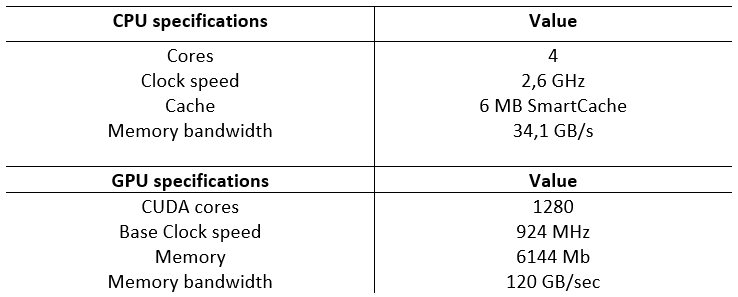
\includegraphics[width=1\textwidth]{figures/Specs}
\caption{Specifications of CPU‘s and GPU [website],[website].}
\label{fig:Specs}
\end{figure}